\section{Sharding}


\subsection{Funcion de creación de datos}
Se utilizo el siguiente código en js, para generar las inserciones de datos, permitiendo definir un total y un tamaño de lote (y una pausa si fuera necesario). La función genera registros para insertar,en este caso únicamente con código postal aleatorio (ya que era lo importante para el ejemplo) e imprime la información provista por los comandos que provee mongodb para reportar el estado del sharding 	\textbf{sh.status()} y \textbf{db.collection.getShardDistribution()}.

\begin{lstlisting}
function insertRandomPersonas(total, tam_intervalo, pausa_seg) {

	var start = new Date().getTime();
	var total_count = total;
	
	var cp_size = 99999 ;
	print ("Inicial");
	sh.status()
	db.personas.getShardDistribution()
	print ("------------------------------------------------------------------------");
	
	while (total_count>0){
		var current_loop = Math.min(total_count, tam_intervalo);
		for (var i = 1; i <= current_loop; i++) {
			
			var randomCP = Math.floor((Math.random() * cp_size) );
		
			db.personas.insert({"nombre" : "Juan Perez" ,"password" : "1234" ,"codigo_postal" : randomCP  ,"genero" : "m" ,	"edad" : 28 ,	"fecha_creacion": "2015-01-01"} )
		}
		total_count = total_count - current_loop;
		var end = new Date().getTime();
		var time = end - start;
		print ("Restantes:"+total_count+" Execution time: " + time);
		sh.status()
		db.personas.getShardDistribution()
		print ("------------------------------------------------------------------------");
		sleep(pausa_seg * 1000);
	}
}
\end{lstlisting}

La llamada para insertar 5000000 registros en rangos de 20000 es la siguiente: 
\begin{lstlisting}
insertRandomPersonas(500000,20000,0);
\end{lstlisting}

\subsection{Pruebas}
Para las pruebas a realizar se configuraron 4 shards de acuerdo al tutorial provisto por la cátedra y se realizaron pruebas primero utilizando un \textit{indice simple} y después (regenerando de cero los shards) un \textit{indice hash}.\\
Se realizaron varias pruebas para cada tipo de indice, sin embargo se provee solo un ejemplo de cada una, ya que los resultados por tipo de indice tuvieron el mismo comportamiento, sin tener exactamente las mismas cantidades insertadas por el componente aleatorio en la insercion. 

\pagebreak

\subsection{Resultados}
\textbf{Indice Simple} \\
\begin{tabular}{ | l | l | l | l | l | }
\hline
	Cant Registros Insertados & Shard1 & Shard2 & Shard3 & Shard4 \\ \hline
	0 & 0 & 0 & 0 & 0 \\ \hline
	20000 & 3441 & 8237 & 8322 & 0 \\ \hline
	40000 & 6925 & 16346 & 16729 & 0 \\ \hline
	60000 & 10362 & 24416 & 25222 & 0 \\ \hline
	80000 & 13829 & 32392 & 33779 & 0 \\ \hline
	100000 & 17128 & 40546 & 42326 & 0 \\ \hline
	120000 & 20478 & 48579 & 50943 & 0 \\ \hline
	140000 & 23888 & 56671 & 59441 & 0 \\ \hline
	160000 & 27289 & 64815 & 67896 & 0 \\ \hline
	180000 & 30705 & 72895 & 38764 & 37636 \\ \hline
	200000 & 34168 & 80927 & 43157 & 41748 \\ \hline
	220000 & 37626 & 88957 & 47486 & 45931 \\ \hline
	240000 & 41100 & 97070 & 51754 & 50076 \\ \hline
	260000 & 44453 & 66860 & 56108 & 92579 \\ \hline
	280000 & 47847 & 72029 & 60453 & 99671 \\ \hline
	300000 & 51300 & 77048 & 64775 & 106877 \\ \hline
	320000 & 54697 & 82171 & 69025 & 114107 \\ \hline
	340000 & 58072 & 87357 & 73420 & 121151 \\ \hline
	360000 & 61526 & 92442 & 77729 & 128303 \\ \hline
	380000 & 65013 & 97555 & 82002 & 135430 \\ \hline
	400000 & 68423 & 102615 & 86393 & 142569 \\ \hline
	420000 & 108673 & 107816 & 53816 & 149695 \\ \hline
	440000 & 113798 & 112928 & 56349 & 156925 \\ \hline
	460000 & 119068 & 117956 & 58953 & 164023 \\ \hline
	480000 & 124353 & 122915 & 61521 & 171211 \\ \hline
	500000 & 129591 & 127964 & 64092 & 178353 \\ \hline
\end{tabular} \\
 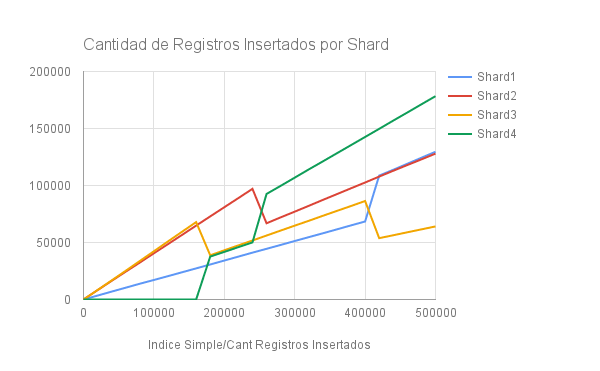
\includegraphics[width=\linewidth]{IndiceSimpleChart.png}
\pagebreak

\textbf{Indice Hash} \\
\begin{tabular}{ | l | l | l | l | l | }
\hline
	Cant Registros Insertados & Shard1 & Shard2 & Shard3 & Shard4 \\ \hline
	0 & 0 & 0 & 0 & 0 \\ \hline
	20000 & 5039 & 4901 & 5067 & 4993 \\ \hline
	40000 & 10170 & 9942 & 9967 & 9921 \\ \hline
	60000 & 15211 & 14962 & 15003 & 14824 \\ \hline
	80000 & 20109 & 20089 & 19971 & 19831 \\ \hline
	100000 & 25155 & 25113 & 24940 & 24792 \\ \hline
	120000 & 30143 & 30194 & 29923 & 29740 \\ \hline
	140000 & 35116 & 35160 & 34950 & 34774 \\ \hline
	160000 & 40093 & 40220 & 39926 & 39761 \\ \hline
	180000 & 45084 & 45172 & 44947 & 44797 \\ \hline
	200000 & 50160 & 50210 & 49953 & 49677 \\ \hline
	220000 & 55212 & 55214 & 54972 & 54602 \\ \hline
	240000 & 60194 & 60226 & 59949 & 59631 \\ \hline
	260000 & 65222 & 65226 & 64931 & 64621 \\ \hline
	280000 & 70210 & 70247 & 69921 & 69622 \\ \hline
	300000 & 75309 & 75162 & 74942 & 74587 \\ \hline
	320000 & 80403 & 80062 & 80020 & 79515 \\ \hline
	340000 & 85527 & 84939 & 84987 & 84547 \\ \hline
	360000 & 90583 & 89902 & 89914 & 89601 \\ \hline
	380000 & 95566 & 94898 & 94837 & 94699 \\ \hline
	400000 & 100428 & 99931 & 99805 & 99836 \\ \hline
	420000 & 105363 & 105137 & 104749 & 104751 \\ \hline
	440000 & 110394 & 110037 & 109801 & 109768 \\ \hline
	460000 & 115318 & 115106 & 114785 & 114791 \\ \hline
	480000 & 120196 & 120176 & 119788 & 119840 \\ \hline
	500000 & 125288 & 125160 & 124708 & 124844 \\ \hline
\end{tabular} \\
 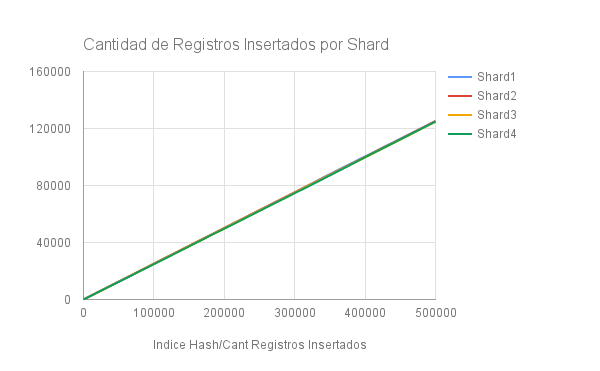
\includegraphics[width=\linewidth]{IndiceHashChart.png}
 
\pagebreak
\subsection{Analisis}

Se puede ver que  utilizando un \textit{indice simple} para un campo en el cual los datos estan generados de manera aleatoria, lo que sucede es que empieza a crecer un shard mas que otros y en algun momento el balanceador decide migrar un subconjunto de estos datos a otro shard menos cargado. Esto se va realizando varias veces durante la carga de datos, de acuerdo al nivel de crecimiento de cada shard.\\
Una vez realizadas las pruebas verificamos cual es el mecanismo utilizado por mongodb en estos casos y esta explicado en la seccion \textbf{Chunk Migration Across Shards} del manual de mongodb. Básicamente decide balancear cuando la diferencia entre la cantidad de \textit{chunks} entre el shard con mas \textit{chunks}  y el shard con menos \textit{chunks} es superior a un valor configurado internamente dentro del balanceador de mongodb.\\
Utilizando un \textit{indice hash} lo que sucede es que los registros generados se van insertando de manera pareja entre todos los shards y en ese caso nunca le hace falta al balanceador hacer una migración de \textit{chunks}.

\subsection{Escenarios posibles para sharding}
Algunos escenarios posibles para sharding son:\\

Tener una base con consultas/visitas de clientes a un sitio web con alta concurrencia, que guarden que items vio, en que esta interesado, historial de navegación, etc. Estas consultas/visitas pueden crecer muy rápidamente y generar un volumen my grande de datos. En este caso una base con mongodb con sharding permitiría un crecimiento acorde al uso que va teniendo la aplicación.Un atributo posible para sharding en este caso es el numero de cliente.\\

Tener una empresa de logística o correo, que quiere mantener una base con el total de envíos de paquetes realizados, en este caso se podría utilizar como atributo de sharding código postal del destinatario, siempre y cuando el envío de paquetes realizados tenga una distribución uniforme ( o lo mas próxima posible a uniforme ) y variada de destinos para los envíos con los que trabaja.En este caso la base podría crecer lo que fuera necesario y sabríamos que tendríamos equilibrada entre todos los shards.\\

Queremos tener una base de datos de usuarios conectados a un juego online de alta concurrencia. Esta base debe guardar información variada de los jugadores y de las partidas mientras están conectados. Esta base puede tener variaciones en la carga dependiendo de los días del horario, día de la semana o época del año (en vacaciones tiene mas uso). En este caso se podría usar el sharding para permitir un crecimiento/decrecimiento de la base de acuerdo a lo que fuera necesario y de manera equilibrada. En este caso podríamos usar como atributo para sharding el id de jugador.\\


\subsection{Características de un atributo para sharding}
Un atributo para ser usado como clave en un esquema de sharding debe tener algunas características:\\

\begin{itemize}		
	\item Alta Cardinalidad: Si un atributo tiene baja cardinalidad no es útil para sharding, ya que todos los registros con el mismo atributo terminan en un mismo chunk y en caso de que uno quisiera tener un numero grande de shards, esta acotado por la cardinalidad de este atributo.
	\item Tener una distribución uniforme: Un atributo debe tener una distribucion uniforme para el dominio del problema en el que se esta trabajando, ya que si no es posible que se llenen mucho algunos shards y otros queden vacios. Por ejemplo utilizar código postal como clave para shard puede ser bueno (inclusive con los balanceos) si tiene una distribución pareja (tenemos personas o clientes de todo el país), sin embargo si nuestra base de clientes es de un solo barrio de una ciudad, la variabilidad de códigos postales puede ser muy acotada.
\end{itemize}
